\documentclass[12pt]{report}
\usepackage[utf8]{inputenc}
\usepackage[russian]{babel}
%\usepackage[14pt]{extsizes}
\usepackage{listings}
\usepackage{graphicx}
\usepackage{amsmath,amsfonts,amssymb,amsthm,mathtools} 
\usepackage{float}

% Для листинга кода:
\lstset{ %
language=C++,                 % выбор языка для подсветки (здесь это С)
basicstyle=\small\sffamily, % размер и начертание шрифта для подсветки кода
numbers=left,               % где поставить нумерацию строк (слева\справа)
numberstyle=\tiny,           % размер шрифта для номеров строк
stepnumber=1,                   % размер шага между двумя номерами строк
numbersep=5pt,                % как далеко отстоят номера строк от подсвечиваемого кода
showspaces=false,            % показывать или нет пробелы специальными отступами
showstringspaces=false,      % показывать или нет пробелы в строках
showtabs=false,             % показывать или нет табуляцию в строках
frame=single,              % рисовать рамку вокруг кода
tabsize=2,                 % размер табуляции по умолчанию равен 2 пробелам
captionpos=t,              % позиция заголовка вверху [t] или внизу [b] 
breaklines=true,           % автоматически переносить строки (да\нет)
breakatwhitespace=false, % переносить строки только если есть пробел
escapeinside={\#*}{*)}   % если нужно добавить комментарии в коде
}

% Для измененных титулов глав:
\usepackage{titlesec, blindtext, color} % подключаем нужные пакеты
\definecolor{gray75}{gray}{0.75} % определяем цвет
\newcommand{\hsp}{\hspace{20pt}} % длина линии в 20pt
% titleformat определяет стиль
\titleformat{\chapter}[hang]{\Huge\bfseries}{\thechapter\hsp\textcolor{gray75}{|}\hsp}{0pt}{\Huge\bfseries}


% plot
\usepackage{pgfplots}
\usepackage{filecontents}
\usetikzlibrary{datavisualization}
\usetikzlibrary{datavisualization.formats.functions}


\begin{document}
%\def\chaptername{} % убирает "Глава"
\begin{titlepage}
	\centering
	{\scshape\LARGE МГТУ им. Баумана \par}
	\vspace{3cm}
	{\scshape\Large Лабораторная работа №4\par}
	\vspace{0.5cm}	
	{\scshape\Large По курсу: "Анализ алгоритмов"\par}
	\vspace{1.5cm}
	{\huge\bfseriesПараллельное умножение матриц\par}
	\vspace{2cm}
	\Large Работу выполнил: Гаврилов Дмитрий, ИУ7-56Б\par
	\vspace{0.5cm}
	\LargeПреподаватели:  Волкова Л.Л., Строганов Ю.В.\par

	\vfill
	\large \textit {Москва, 2019} \par
\end{titlepage}

\tableofcontents

\newpage
\chapter*{Введение}
\addcontentsline{toc}{chapter}{Введение}
Цель работы: изучение алгоритмов умножения матриц. В данной лабораторной работе рассматривается стандартный алгоритм умножения матриц, алгоритм Винограда и модифицированный алгоритм Винограда.  Также требуется изучить рассчет сложности алгоритмов, получить навыки в улучшении алгоритмов.
Эти алгоритмы активно применяются во всех областях, применяющих линейную алгебру, таких как:
\begin{itemize}
	\item компьютерная графика
	\item физика
	\item экономика
\end{itemize}


В ходе лабораторной работы предстоит:
\begin{itemize}
	\item  Изучение и реализация параллельного алгоритма Винограда для умножения матриц 
	\item Сравнить зависимость времени работы алгоритма от числа параллельных потоков исполнения и размера матриц 
	\item Провести сравнение стандартного и параллельного алгоритма.
\end{itemize}


\chapter{Аналитическая часть}
Матрицей A размера $[m*n]$ называется прямоугольная таблица
чисел, функций или алгебраических выражений, содержащая m строк и n столбцов. Числа m и n определяют размер матрицы.\cite{Beloysov} Если число столбцов в первой матрице совпадает с числом строк во второй, то эти две матрицы можно перемножить. У произведения будет столько же строк, сколько в первой матрице, и столько же столбцов, сколько во второй.
	    
Пусть даны две прямоугольные матрицы А и В размеров $[m * n]$ и $[n * k]$ соответственно.  
В результате произведение матриц A и B получим матрицу C размера $[m *  k]$.

$C_{i,j} = \sum\limits_{r=1}^n A_{i,r}\cdot B_{r,j}$ называется произведением матриц A и B \cite{Beloysov}.


\section{Алгоритм Винограда}
Подход Алгоритма Винограда является иллюстрацией общей методологии, начатой в 1979-х годах на основе
билинейных и трилинейных форм, благодаря которым большинство усовершенствований для умножения матриц были получены \cite{Gall2012}.

Рассмотрим два вектора $V = (v1, v2, v3, v4)$ и $W = (w1, w2, w3, w4)$.  

 Их скалярное произведение равно (\ref{formula}) 

\begin{equation} \label{formula}
V \cdot W=v_1 \cdot w_1 + v_2 \cdot w_2 + v_3 \cdot w_3 + v_4 \cdot w_4
\end{equation}

Равенство (\ref{formula}) можно переписать в виде (\ref{formula2}) 
\begin{equation} \label{formula2}
V \cdot W=(v_1 + w_2) \cdot (v_2 + w_1) + (v_3 + w_4) \cdot (v_4 + w_3) - v_1 \cdot v_2 - v_3 \cdot v_4 - w_1 \cdot w_2 - w_3 \cdot w_4
\end{equation}

Выражение в правой части последнего равенства допускает предварительную обработку: его части можно вычислить заранее и запомнить для каждой строки первой матрицы и для каждого столбца второй. 
Это означает, что над предварительно обработанными элементами нам придется выполнять лишь первые два умножения и последующие пять сложений, а также дополнительно два сложения. 

В алгоритме Винограда, результатом умножение матриц A размером $[m * n]$ и B размером $[n * k]$ получим матрицу C размера $[m *  k]$ которая вычисляется по следующим формулам:

Вычисление строковых множителей (\ref{rowFactors})
\begin{equation} \label{rowFactors}
Rows_{i} = \sum\limits_{j = 1}^{n/2} A_{i, 2j} \cdot A_{i, 2j+1}
\end{equation}

Вычисление множителей стобцов (\ref{columnFactors})
\begin{equation} \label{columnFactors}
Cols_{i} = \sum\limits_{j = 1}^{n/2} B_{2j, i} \cdot B_{2j+1, i}
\end{equation}

Вычисление результирующей матрицы С (\ref{result})
\begin{equation} \label{result}
C_{i,j} = -Rows_{i} -  Cols_{j} + \sum\limits_{k = 1}^{n/2} (A_{i, 2k+1} + B_{2k, j}) \cdot (A_{i, 2k} + B_{2k+1,j})
\end{equation}

Следует отметить, что в худшем случае (при условии того что кол-во столбцев в матрице А либо кол-во строк в матрице В - нечётное) к результирующей формуле (\ref{result}) применяется следующее выражение (\ref{resultBad})

\begin{equation} \label{resultBad}
C_{i,j} += A_{i, n} \cdot B_{n, j}
\end{equation}

\section{Параллельный алгоритм Винограда }
Трудоемкость алгоритма Винограда имеет сложность $O(nmk)$ для умножения матриц $n1 \times m1$ на $n2 \times m2$. Чтобы улучшить алгоритм, следует распараллелить ту часть алгоритма, которая содержит 3 вложенных цикла.\\

	Вычисление результата для каждой строки не зависит от результата выполнения умножения для других строк. Поэтому можно распараллелить часть кода, где происходят эти действия. Каждый поток будет выполнять вычисления определенных строк результирующей матрицы.
	
\section{Распараллеливание задачи}
В рамках данной лабораторной работы производилось распараллеливание задачи по потокам. В CPU для данной цели используются tread.  \\
	
	CPU – central processing unit – это универсальный процессор, также именуемый процессором общего назначения. Он оптимизирован для достижения высокой производительности единственного потока команд. Доступ к памяти с данными и инструкциями происходит преимущественно случайным образом.
Для того, чтобы повысить производительность CPU еще больше, они проектируются специально таким образом, чтобы выполнять как можно больше инструкций параллельно. Например для этого в ядрах процессора используется блок внеочередного выполнения команд.	
Но несмотря на это, CPU все равно не в состоянии осуществить параллельное выполнение большого числа инструкций, так как расходы на распараллеливание инструкций внутри ядра оказываются очень существенными. Именно поэтому процессоры общего назначения имеют не очень большое количество исполнительных блоков.
Реальную многопоточность можно обеспечить, если количество созданных потоков в программе будет равным количеству логических ядер процессора.
В рамках данной работы будет выполнено распарралеливании задачи для процессора который имеет 4 логических ядра.


\subsection{Вывод}
Были рассмотрены стандартная и параллельная реализации алгоритма Винограда.


\chapter{Конструкторская часть}
\textbf{Требования к вводу:}\\
На вход подаются две матрицы и их размерности\\
\textbf{Требования к программе:}\\
Корректное умножение двух матриц \\


\section{Схемы алгоритмов}

На рис. \ref{fig:def} представлена  схема стандартного алгоритма Винограда:
	\begin{figure}[h]
        	\begin{center}
        		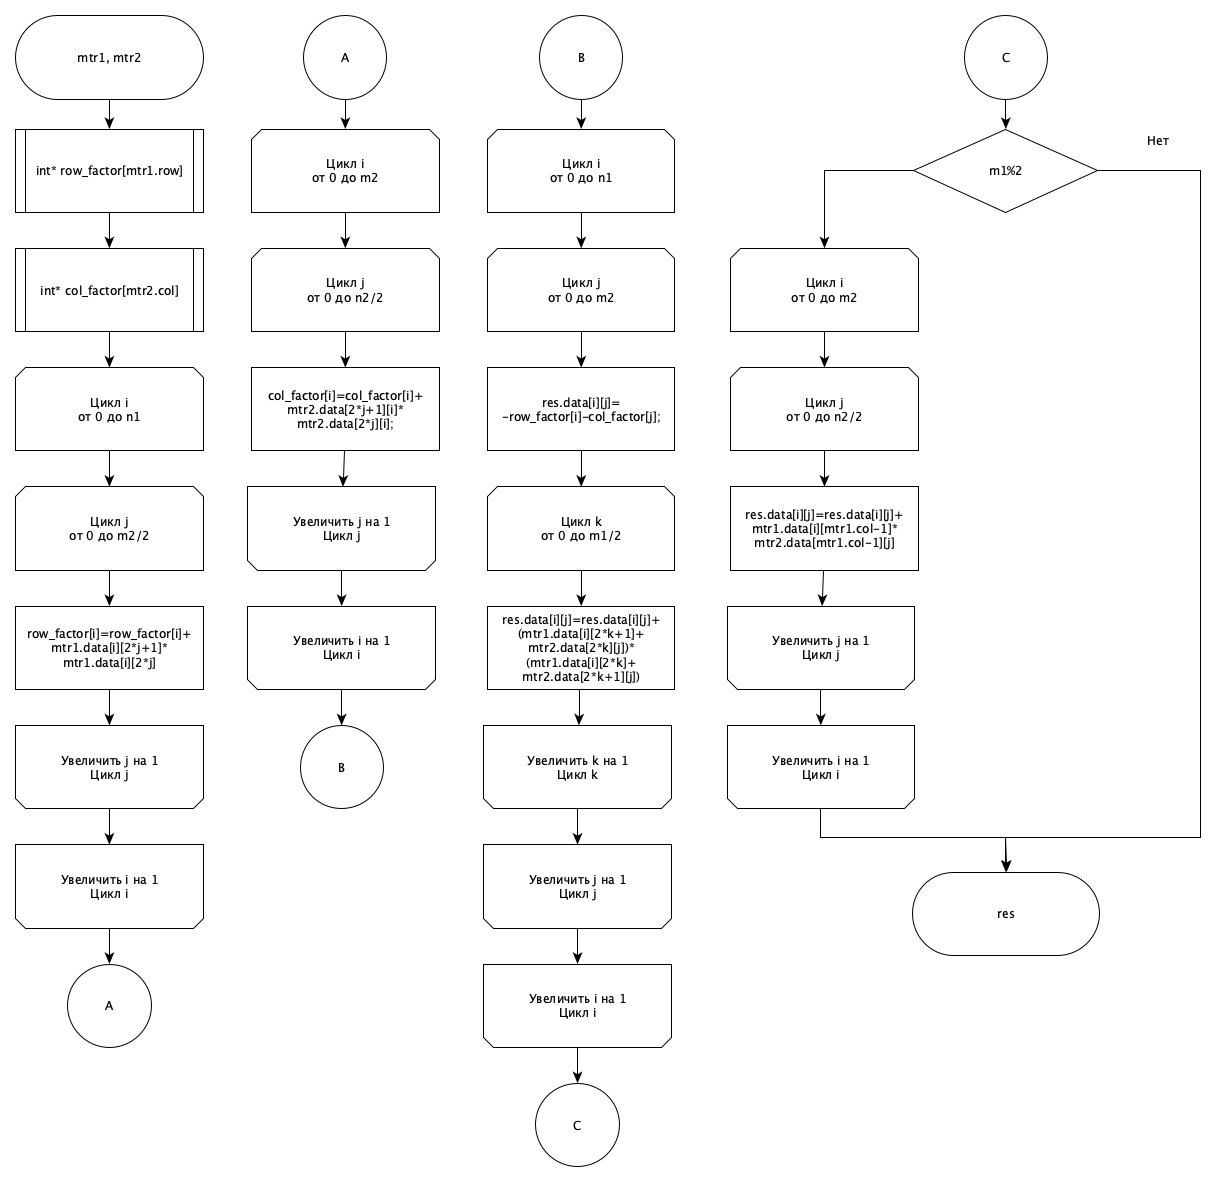
\includegraphics[scale=0.32]{standart_vinograd2}
        		\caption{Cхема стандартного алгоритма Винограда}
        		\label{fig:def}
        	\end{center}
        \end{figure}
        
На рис. \ref{fig:def} представлена схема распараллеленого алгоритма Винограда:
	\begin{figure}[h]
        	\begin{center}
        		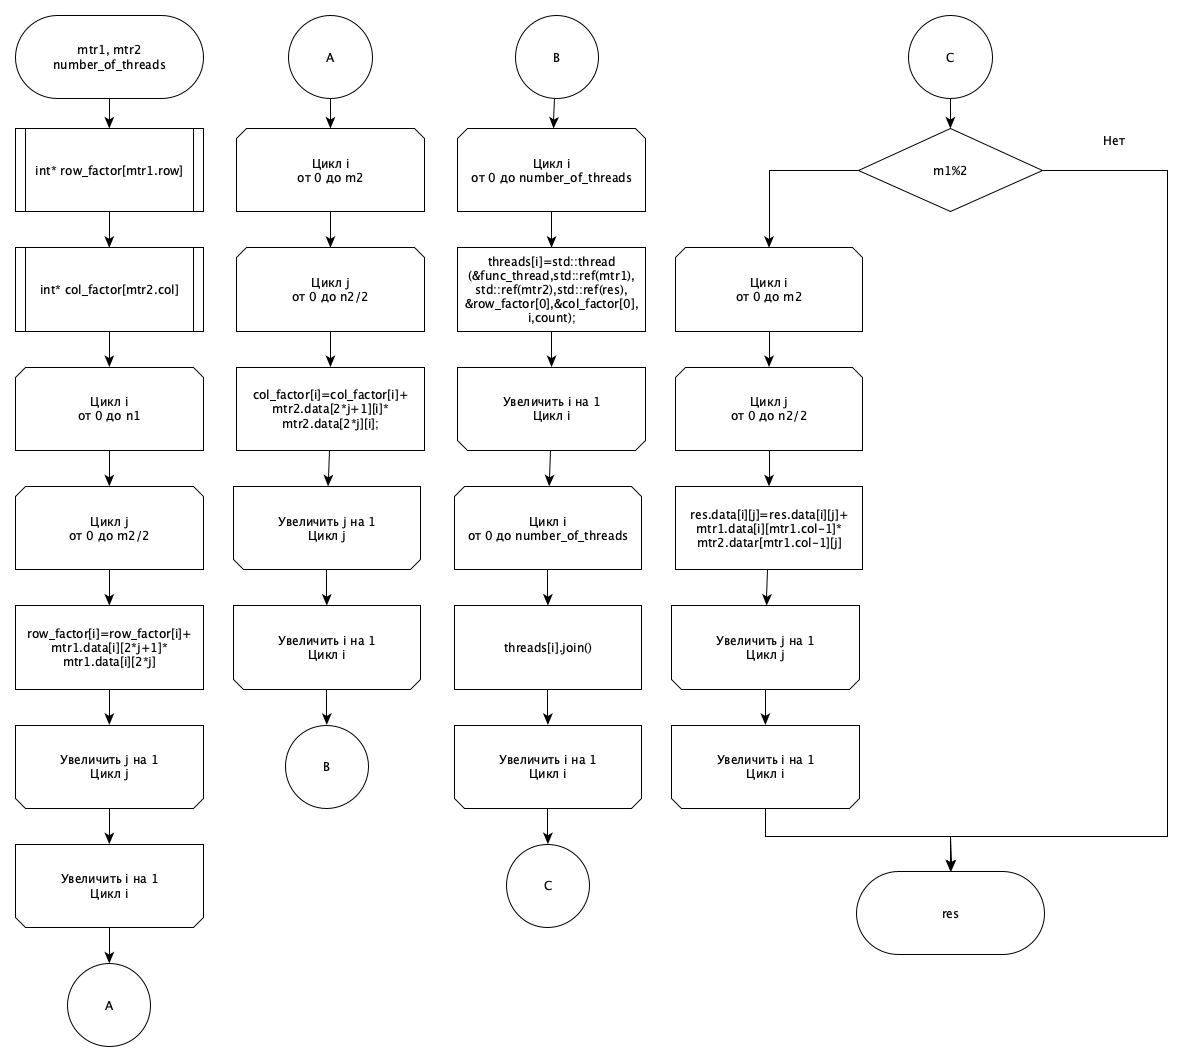
\includegraphics[scale=0.32]{parallel_vinograd2}
        		\caption{Схема распараллеленого алгоритма Винограда}
        		\label{fig:def}
        	\end{center}
        \end{figure}
        
На рис. \ref{fig:def} ппредставлена схема фнкции параллельного вычисления матрицы:
	\begin{figure}[h]
        	\begin{center}
        		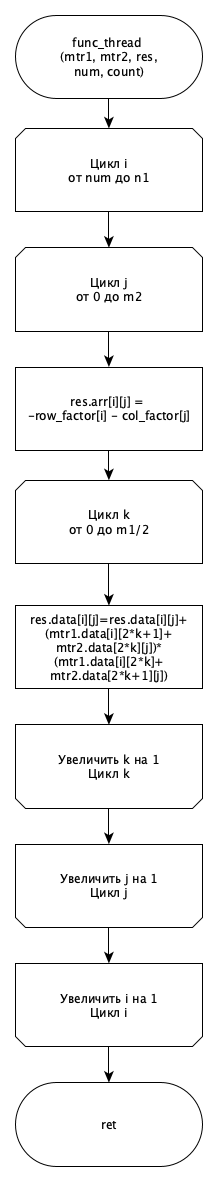
\includegraphics[scale=0.32]{parallel_func}
        		\caption{Схема функции выполняющей парралельные вычисления}
        		\label{fig:def}
        	\end{center}
        \end{figure}

\chapter{Технологическая часть}
\section{Выбор ЯП}
Для реализации программ я выбрал язык программирования Java, так имею большой опыт работы с ним. Среда разработки - IntelliJ IDEA. \\

Для работы с потоками используется библиотека поддержки потоков java.util.concurrent. \\
Для замера времени используется системный вызов System.currentTimeMillis, возвращающий количество миллисекунд.\\


\section{Реализация алгоритма}
В листинге \ref{s} будет рассмотрина реализация стандартного алгоритма Винограда

\begin{lstlisting}[label=s,caption=Стандартный алгоритм Винограда]
public class MultiplyVinograd implements MatrixMultiplier {
    @Override
    public int[][] multiply(int[][] firstMatrix, int[][] secondMatrix) {
        int firstRowCount = firstMatrix.length;
        int secondRowCount = secondMatrix.length;

        if (firstRowCount == 0 || secondRowCount == 0)
            return null;

        int firstColumnCount = firstMatrix[0].length;
        int secondColumnCount = secondMatrix[0].length;

        if (firstColumnCount != secondRowCount)
            return null;

        int[] rowFactors = new int[firstRowCount];
        int[] columnFactors = new int[secondColumnCount];

        int[][] result = new int[firstRowCount][secondColumnCount];

        for (int i = 0; i < firstRowCount; i++) {
            for (int j = 0; j < firstColumnCount / 2; j++) {
                rowFactors[i] += firstMatrix[i][j * 2] * firstMatrix[i][j * 2 + 1];
            }
        }

        for (int i = 0; i < secondColumnCount; i++) {
            for (int j = 0; j < secondRowCount / 2; j++) {
                columnFactors[i] += secondMatrix[j * 2][i] * secondMatrix[j * 2 + 1][i];
            }
        }

        for (int i = 0; i < firstRowCount; i++) {
            for (int j = 0; j < secondColumnCount; j++) {
                result[i][j] = -rowFactors[i] - columnFactors[j];
                for (int k = 0; k < firstColumnCount / 2; k++) {
                    result[i][j] += (firstMatrix[i][2 * k + 1] + secondMatrix[2 * k][j]) * (firstMatrix[i][2 * k] + secondMatrix[2 * k + 1][j]);
                }
            }
        }

        if (firstColumnCount \% 2 == 1) {
            for (int i = 0; i < firstRowCount; i++) {
                for (int j = 0; j < secondColumnCount; j++) {
                    result[i][j] += firstMatrix[i][firstColumnCount - 1] * secondMatrix[firstColumnCount - 1][j];
                }
            }
        }

        return result;
    }
}
\end{lstlisting}



	
	Можно заметить, что вычисление результата для каждой строки происходит независимо от результата выполнения умножения для других строк. Поэтому возможно распараллелить участок кода, соответстующий строкам 33-40 листинга \ref{s}. Каждый поток будет выполнять вычисление некоторых строк результирующей матрицы. Это сделано потому, что проход по строкам матрицы является более эффективным с точки зрения организации данных в памяти.

В листинге \ref{p} представлен параллельный алгоритм Винограда:\\

	\begin{lstlisting}[label=p,caption=Параллельный алгоритм Винограда]
public class MultiplyVinogradParralel{
    public int[][] multiplyParralel(int[][] firstMatrix, int[][] secondMatrix, int threadsCount) throws InterruptedException {
        int firstRowCount = firstMatrix.length;
        int secondRowCount = secondMatrix.length;

        if (firstRowCount == 0 || secondRowCount == 0) {
            return null;
        }

        int firstColumnCount = firstMatrix[0].length;
        int secondColumnCount = secondMatrix[0].length;

        if (firstColumnCount != secondRowCount) {
            return null;
        }

        int[] rowFactors = new int[firstRowCount];
        int[] columnFactors = new int[secondColumnCount];

        int[][] result = new int[firstRowCount][secondColumnCount];

        for (int i = 0; i < firstRowCount; i++) {
            for (int j = 0; j < firstColumnCount / 2; j++) {
                rowFactors[i] += firstMatrix[i][j * 2] * firstMatrix[i][j * 2 + 1];
            }
        }

        for (int i = 0; i < secondColumnCount; i++) {
            for (int j = 0; j < secondRowCount / 2; j++) {
                columnFactors[i] += secondMatrix[j * 2][i] * secondMatrix[j * 2 + 1][i];
            }
        }

        ExecutorService service = Executors.newFixedThreadPool(threadsCount);


        for (int i = 0; i < threadsCount; i++) {
            service.execute(new LoopExecutor(
                    firstMatrix,
                    secondMatrix,
                    result,
                    rowFactors,
                    columnFactors,
                    i,
                    threadsCount));
        }
        service.shutdown();

        while (!service.awaitTermination(24L, TimeUnit.HOURS)) {
            System.out.println("Not yet. Still waiting for termination");
        }


        if (firstColumnCount \% 2 == 1) {
            for (int i = 0; i < firstRowCount; i++) {
                for (int j = 0; j < secondColumnCount; j++) {
                    result[i][j] += firstMatrix[i][firstColumnCount - 1] * secondMatrix[firstColumnCount - 1][j];
                }
            }
        }

        return result;
    }
}
\end{lstlisting}

В листинге \ref{pf} представлено распараллеленное вычисление тройного цикла:

	\begin{lstlisting}[label=pf,caption=Распараллеленный тройной цикл]
class LoopExecutor implements Runnable {
        private int[][] firstMatrix;
        private int[][] secondMatrix;
        private int[][] result;
        private int[] rowFactors;
        private int[] colFactors;
        private int startIndex;
        private int step;

        public LoopExecutor(int[][] firstMatrix, int[][] secondMatrix, int[][] result, int[] rowFactors, int[] colFactors, int startIndex, int step) {
            this.firstMatrix = firstMatrix;
            this.secondMatrix = secondMatrix;
            this.result = result;
            this.rowFactors = rowFactors;
            this.colFactors = colFactors;
            this.startIndex = startIndex;
            this.step = step;
        }

        @Override
        public void run() {
            for (int i = startIndex; i < firstMatrix.length; i+=step) {
                for (int j = 0; j < secondMatrix[0].length; j++) {
                    result[i][j] = -rowFactors[i] - colFactors[j];
                    for (int k = 0; k < firstMatrix[0].length / 2; k++) {
                        result[i][j] += (firstMatrix[i][2 * k + 1] + secondMatrix[2 * k][j]) * (firstMatrix[i][2 * k] + secondMatrix[2 * k + 1][j]);
                    }
                }
            }
        }
    }
\end{lstlisting}



\chapter{Исследовательская часть}

\section{Постановка эксперимента}

Были проведены исследования зависимости времени работы трех алгоритмов от размеров перемножаемых матриц и количества использованных потоков. Замеры времени проводились для матриц четной размерности размером от 100 до 1000 с шагом 100 и матриц нечетной размерности размером от 101 до 1001 с шагом 100. Количество потоков - от 1 до 16, т.к. компьютер, на котором проводились вычисления, содержит 4 логических ядра.\\
	
	 Временные замеры проводятся путём многократного проведения эксперимента и деления результирующего времени на количество итераций эксперимента. \\

\section{Сравнительный анализ на основе замеров времени работы алгоритмов}

На рис. 4.1 представлен график времени работы алгоритма на матрицах четной размерности:
	
\begin{tikzpicture}
\begin{axis}[
    	axis lines = left,
    	xlabel = Размер матрицы,
    	ylabel = Время (мс),
	legend pos=north west,
	ymajorgrids=true
]
\addplot[color=red, mark=square] table[x index=0, y index= 1] {NoThreadsEven.txt}; 
\addplot[color=blue, mark=square] table[x index=0, y index= 1] {OneThreadEven.txt}; 
\addplot[color=green, mark=square] table[x index=0, y index= 1] {TwoThreadsEven.txt}; 
\addplot[color=yellow, mark=square] table[x index=0, y index= 1] {FourThreadsEven.txt}; 
\addplot[color=brown, mark=square] table[x index=0, y index= 1] {EightThreadsEven.txt}; 
\addplot[color=cyan, mark=square] table[x index=0, y index= 1] {SixteenThreadsEven.txt}; 


\addlegendentry{No threads}
\addlegendentry{One thread}
\addlegendentry{Two threads}
\addlegendentry{Four threads}
\addlegendentry{Eight threads}
\addlegendentry{Sixteen threads}
\end{axis}
\end{tikzpicture}
\begin{center}
Pис. 4.1: Сравнение времени на матрицах чётной размерности
\end{center}

На рис. 4.2 представлен график времени работы алгоритма на матрицах четной размерности:

\begin{tikzpicture}
\begin{axis}[
    	axis lines = left,
    	xlabel = Размер матрицы,
    	ylabel = Время (мс),
	legend pos=north west,
	ymajorgrids=true
]
\addplot[color=red, mark=square] table[x index=0, y index= 1] {NoThreadsOdd.txt}; 
\addplot[color=blue, mark=square] table[x index=0, y index= 1] {OneThreadOdd.txt}; 
\addplot[color=green, mark=square] table[x index=0, y index= 1] {TwoThreadsOdd.txt}; 
\addplot[color=yellow, mark=square] table[x index=0, y index= 1] {FourThreadsOdd.txt}; 
\addplot[color=brown, mark=square] table[x index=0, y index= 1] {EightThreadsOdd.txt}; 
\addplot[color=cyan, mark=square] table[x index=0, y index= 1] {SixteenThreadsOdd.txt}; 


\addlegendentry{No threads}
\addlegendentry{One thread}
\addlegendentry{Two threads}
\addlegendentry{Four threads}
\addlegendentry{Eight threads}
\addlegendentry{Sixteen threads}
\end{axis}
\end{tikzpicture}
\begin{center}
Pис. 4.2: Сравнение времени на матрицах нечётной размерности
\end{center}
	
        

\section{Вывод}

Эксперименты замера времени показали, что при последовательной и параллельной (с одним рабочим потоком) реализациях оптимизированного алгоритма Винограда совсем немного выигрывает последовательная реализация (в ней не тратится время на выделение рабочего потока).
       
        При сравнении замеров времени для параллельной реализации алгоритма с 1, 2, 4, 8 и 16 рабочими потоками выяснилось, что максимальная производительность достигается на 8-ми и 16-и рабочих потоках. Выполнение алгоритма на 8-ми рабочих потоках быстрее в 3,82 раз, по сравнению с выполнением на 1-м потоке для матриц размера $1000 \times 1000$.


\chapter*{Заключение}
\addcontentsline{toc}{chapter}{Заключение}
В ходе работы был изучен параллельный алгоритм умножения матриц: алгоритм Винограда. Выполнено сравнение зависимости всех рассматриваемых алгоритмов от числа параллельных потоков и размера матриц. В ходе исследования было установлено, что многопоточный алгоритм Винограда выполняется быстрее, чем стандартный алгоритм.

\end{document}